\par En el documento ``Alternativas de Solución de Proyecto de Titulación''\cite{Gonzalez2020AlternativasTitulacion} se presentaron 4 posibles alternativas para la implementación de un sistema de adquisición de datos para detectores de muones. En cada una de ellas se proponen distintas tecnologías para llevar acabo el mismo fin: Digitizers, Microcontroladores, CPLDs y FPGAs. La figura \ref{fig:diagrama} ilustra la estructura general del sistema de adquisicón de datos. 
\par En el actual documento se presenta el contraste entre las 4 alternativas discutidas con anterioridad, asignando puntaciones a cada una de ellas en base a criterios clave asociados a las características y el diseño del sistema. Los criterios a evaluar son: simplicidad, desempeño, disponibilidad, economía, flexibilidad y documentación. La comparativa que se desarrolla aquí tiene como objetivo definir cuál de las 4 opciones es la mejor alternativa a desarrollar, cumpliendo además con los requisitos principales del proyecto.
\par La alternativa seleccionada se presenta y detalla a continuación de la comparación de alternativas, planteando sus características principales y justificando la elección realizada.
%\begin{figure}[H]
%    \centering
%    
%    \tikzstyle{externo} = [rectangle, rounded corners, minimum width=2cm, minimum height=1cm,text centered, draw=black, fill=blue!30]
%    \tikzstyle{fpga} = [rectangle, rounded corners, minimum width=3cm, minimum height=2.5cm,text centered, draw=black, fill=green!30]
%    \tikzstyle{flecha} = [thick,->,>=stealth]   
%    
%    \begin{tikzpicture}[node distance=1.5cm]
%
%        \node (disparo) [externo] {Disparo};
%        \node (detector) [externo, below of=disparo] {Detector};
%        \node (asd) [externo, right of=detector, xshift=1cm] {ASD};
%        \node (disc) [fpga, right of=detector, xshift=2.5cm, yshift=-0.5cm, anchor=south west] {Discriminador};
%        \node (pros) [fpga, right of=disc, xshift=2cm] {Procesamiento};
%        \node (res) [fpga, right of=pros, xshift=2cm] {Análisis};
%        
%        \draw [flecha] (disparo) --  (disc.west |- disparo);
%        \draw [flecha] (detector) -- (asd);
%        \draw [flecha] (asd) -- (disc.west |- asd);
%        \draw [flecha] (disc) -- (pros);
%        \draw [flecha] (pros) -- (res);
%
%    \end{tikzpicture}
%
%    \caption{Diagrama de bloques del sistema. En azul se presentan las etapas previas al proyecto que ya se encuentran desarrolladas y sobre las cuales no se tiene control. En verde se ilustran las etapas pendientes y que pueden ser desarrolladas en este proyecto. El disparo corresponde a la señal digital que indica si la partícula detectada es un muón y el ASD es un acondicionador de señal que genera pulsos digitales a partir de los pulsos analógicos captados.}
%    \label{fig:diagrama}
%\end{figure}


\section{Criterios de Selección}
\par Para seleccionar la alternativa más adecuada se definieron seis distintos criterios de evaluación, cada uno de los cuales puede obtener un puntaje entre 1 y 10. Los criterios tienen distinta relevancia dentro del proyecto, resultando en que algunos de ellos tengan mayor ponderación respecto a otros. La tabla \ref{tab:criterios} indica el porcentaje de relevancia correspondiente cada criterio de selección. 

\begin{table}[H]
\centering
\begin{tabular}{|l|c|}
\hline
\textbf{Criterio de Selección} & \textbf{Porcentaje de Relevancia} \\ \hline
Simplicidad & 10\% \\ \hline
Desempeño & 35\% \\ \hline
Disponibilidad & 25\% \\ \hline
Economía & 10\% \\ \hline
Flexibilidad & 10\% \\ \hline
Documentación & 10\% \\ \hline
\textit{Total} & \textit{100\%} \\ \hline
\end{tabular}
\caption{Porcentaje de relevancia para cada criterio.}
\label{tab:criterios}
\end{table}

\newpage
\par Se considera como criterio de mayor importancia al \textit{desempeño} estimado de la alternativa, ya que será el aspecto que defina la calidad y funcionamiento del sistema. En segundo lugar de relevancia se ubica la \textit{disponibilidad} de recursos, ya que sin ellos no es posible construir el dispositivo. Los criterios restantes se consideraron menor con ponderación ya que son importantes, pero no cruciales para llevar a cabo el proyecto en su primera versión.
\par Cada criterio es evaluado con un puntaje de 1 a 10 puntos en una escala indicada en la tabla \ref{tab:escala}. A continuación se detalla cada criterio, incluyendo su descripción y explicando la interpretación de puntaje según la escala mencionada.

\begin{table}[H]
\centering
\begin{tabular}{lllll}
\hline
\multicolumn{1}{|c|}{\textbf{Muy Baja}} & \multicolumn{1}{c|}{\textbf{Baja}} & \multicolumn{1}{c|}{\textbf{Media}} & \multicolumn{1}{c|}{\textbf{Alta}} & \multicolumn{1}{c|}{\textbf{Muy Alta}} \\ \hline
\multicolumn{1}{|c|}{1 - 2}                 & \multicolumn{1}{c|}{3 - 4}             & \multicolumn{1}{c|}{5 - 6}           & \multicolumn{1}{c|}{7 - 8}           & \multicolumn{1}{c|}{9 - 10}              \\ \hline 
\end{tabular}
\caption{Tabla de puntajes para criterios de evaluación.}
\label{tab:escala}
\end{table}

\subsection*{Simplicidad}
\par El criterio de simplicidad se refiere a la dificultad de diseñar, programar, fabricar y ensamblar el sistema descrito en la alternativa evaluada. La máxima simplicidad está indicada con un puntaje 10 y la mínima simplicidad con un puntaje 1. Máxima simplicidad implica conectar elementos sin mayor esfuerzo, prácticamente no programar software y prácticamente no diseñar ni implementar hardware. Mínima simplicidad implicaría dificultad de interconexión entre elementos componentes, debido a sus estándares o cantidad de conexiones presentes, incluyendo software de alta complejidad y prácticamente el desarrollo completo del hardware.

\subsection*{Desempeño}
La evaluación por desempeño tiene directa relación con los requisitos de diseño asociados al sistema a desarrollar. Estos requisitos son los siguientes:

\begin{itemize}
    \item Se debe contar con al menos 32 pares de entradas bajo el estándar LVDS, con el fin de conectar al menos 2 tarjetas ASD (Amplificator Shaper Discriminator) utilizadas cada una como la interfaz de detectores de 16 canales.
    \item Es importante contar con un reloj presente o sintetizable de una frecuencia mayor a 100[MHz], lo más cercano a 1[GHz] posible, con el fin de captar la duración de los pulsos y el momento de aparición de un evento con la mayor precisión disponible.
    \item Se debe considerar que la señal de disparo que entrará al sistema estará desfasada cerca de 100[ns] respecto al paso real de los muones por el detector, siendo necesaria la implementación de retardos para las señales capturadas o un sistema capaz de distinguir la ocurrencia de eventos y disparos en el tiempo.
    \item  Se debe tener la capacidad de mantener señales sincronizadas, guardar información en memorias temporales y llevar cuenta del transcurso del tiempo entre eventos.
    \item Es requisito que la implementación de la alternativa permita escalamiento para agregar nuevos detectores adyacentes con el fin de aumentar el área de prueba, así como también sincronizarse con detectores paralelos para trazar trayectorias de las partículas captadas.
\end{itemize}

\par Sintetizando estos requisitos, es posible acotarlos a  5 elementos esenciales: número de canales, disponibilidad de puertos LVDS, frecuencia de reloj, implementación o manejo de retardos y recursos de almacenamientos o procesamiento disponibles. La escalabilidad queda implícitamente evaluada con los criterios de simplicidad, economía y flexibilidad.

\par Considerando lo anterior, se le asignará puntaje a este criterio en función de la cantidad de requisitos que cumpla y la calidad con la que sean satisfechos, considerando 10 puntos en caso de cumplir a cabalidad con todos ellos, y asignándole 1 punto en caso de cumplir ninguno.

\subsection*{Disponibilidad}
\par El criterio de disponibilidad evalúa la presencia inmediata de los materiales necesarios para la implementación del sistema. Pondera la cantidad de elementos necesarios como un total de 10 puntos repartidos en cada uno de los elementos componentes para construir un sistema de adquisición de 32 canales. Si un sistema requiere de 5 elementos discretos, tendrá entonces 10 puntos en caso de contar con la disponibilidad de los 5 elementos necesarios. Si alguno no está disponible y requiere ser adquirido, entonces implicaría un descuento de 2 puntos en dicho ejemplo.

\subsection*{Economía}
\par El criterio de economía evalúa el precio total de construcción del dispositivo, incluyendo todo el hardware necesario para la discriminación, procesamiento y análisis, sin considerar un computador en las etapas finales de análisis o recolección de información. Este criterio es útil para contrastar la factibilidad de escalamiento. Un sistema muy costoso implicará dificultades para replicarlo.
\par Su puntaje se asigna considerando cero puntos para un sistema que supere los US\$1000 para implementar 32 canales. Se otorga un máximo de 10 puntos si el sistema tiene un costo menor o igual a US\$60.

\subsection*{Flexibilidad}
\par La flexibilidad es un criterio que representa qué tan adaptable es el sistema en caso de requerir modificaciones. Puede separarse en tres elementos constitutivos: adquisición, procesamiento y análisis. El puntaje se asigna cualitativamente en función de la flexibilidad de la tecnología involucrada en dicha etapa.
\par El puntaje máximo del criterio de flexibilidad son 10 puntos, considerando aproximadamente 3.3 puntos como máximo para cada elemento constitutivo.

\subsection*{Documentación}
\par El criterio de documentación evalúa la disponibilidad de material bibliográfico, tutoriales y ejemplos para la utilización del software y el hardware propio del sistema, así como de las herramientas necesarias para su implementación. Su puntaje se asigna cualitativamente según la misma tabla \ref{tab:escala}.

\newpage
\section{Evaluación de Alternativas}
\label{evaluacion}
\par A continuación se detallan las evaluaciones para cada una de las 4 alternativas propuestas, incluyendo una breve descripción por cada criterio.
\subsection{Digitizer}
\begin{itemize}
    \item \textbf{Simplicidad:} \textit{5 - Media}. Requiere la fabricación de una PCB de interfaz y la integración de 3 aparatos distintos (Digitalizador, interfaz y computador).
    \item \textbf{Desempeño:} \textit{4 - Bajo}. Baja tasa de muestreo, 62.5[MS/s].
    \item \textbf{Disponibilidad:} \textit{2 - Muy Baja}. Se cuenta con un digitalizador, pero no está disponible una interfaz LVDS a TTL ni los retardos necesarios.
    \item \textbf{Economía:} \textit{1 - Muy Baja}. El costo de  un  digitalizador podría superar los US\$1000.
    \item \textbf{Flexibilidad:} \textit{5 - Media}. Alta flexibilidad en análisis ya que se realiza en un computador. También existe flexibilidad en la manera de procesar y estructurar los datos obtenidos. No existe suficiente flexibilidad en la manera de tomar muestras.
    \item \textbf{Documentación:} \textit{6 - Media} Existe documentación, librerías y programas para operar el digitalizador, pero no son las suficientes para tener el dominio total del dispositivo.
\end{itemize}

\subsection{Microcontrolador}
\begin{itemize}
    \item \textbf{Simplicidad: } \textit{2 - Baja}. Gran cantidad de dispositivos, al ser necesario al menos dos microcontroladores por canal y un tercero para unificar datos provenientes de un mismo detector.
    \item \textbf{Desempeño: } \textit{4 - Bajo}. Bajas tasas de muestreo y operación. Requiere conversores LVDS-TTL y retardos.
    \item \textbf{Disponibilidad: } \textit{1 - Baja}. Todos los materiales tendrían que ser adquiridos.
    \item \textbf{Economía: } \textit{6 - Media}, medianamente económico. Si bien las tarjetas de desarrollo pueden ser de bajo costo, se necesitan varias y se agregan componentes extra que aumentan el costo considerablemente. Mejorar la frecuencia de muestreo también incrementa el costo.
    \item \textbf{Flexibilidad:} \textit{5 - Media}. Alta flexibilidad en análisis y en la manera de procesar y estructurar los datos obtenidos. No existe suficiente flexibilidad en la manera de tomar muestras.
    \item \textbf{Documentación:} \textit{6 - Media} Existe documentación, librerías y programas de ejemplo, pero queda sujeto a los microcontroladores que eventualmente se escojan.
\end{itemize}

\newpage
\subsection{CPLD}
\begin{itemize}
    \item \textbf{Simplicidad:} \textit{7 - Alta}. Pocos dispositivos involucrados, solo una CPLD por detector.
    \item \textbf{Desempeño:}  \textit{7 - Alto}. Escasos recursos lógicos y periféricos, pero alta velocidad de reloj (400MHz máximo), opciones para manejar ratardos y cuenta con puertos LVDS.
    \item \textbf{Disponibilidad:} \textit{9 - Alta}. Se cuenta con una de estas tarjetas en el laboratorio.
    \item \textbf{Economía: } \textit{10 - Alta}. Una de estas tarjetas tiene un valor cercano a los US\$30.
    \item \textbf{Flexibilidad:} \textit{10 - Alta}. Alta flexibilidad en análisis, procesamiento y adquisición.
    \item \textbf{Documentación:} \textit{4 - Baja} Existe documentación, pero es poca y no es simple. Existen pocos ejemplos en internet dado que es un fabricante menos conocido y poco aplicado en este tipo de desarrollos. La herramienta de descripción de hardware es similar a las conocidas, pero propia del fabricante.
\end{itemize}


\subsection{FPGA}
\begin{itemize}
    \item \textbf{Simplicidad:}  \textit{6 - Media}. Gran cantidad del sistema concentrado en una sola placa, pero aumenta la dificultad en la descripción de hardware.
    \item \textbf{Desempeño:}  \textit{9 - Alto}. Gran cantidad de recursos lógicos, de almacenamiento y con alta  frecuencia de operación (600MHz máximo).
    \item \textbf{Disponibilidad: } \textit{9 - Alta}. Se cuenta con una en el laboratorio, pero se necesitarán un par de elementos para interconectarla con la placa ASD.
    \item \textbf{Economía: }\textit{6 - Media}. Una tarjeta de desarrollo de este estilo tiene un costo de aproximadamente US\$400.
    \item \textbf{Flexibilidad:} \textit{10 - Alta}. Alta flexibilidad en análisis, procesamiento y adquisición.
    \item \textbf{Documentación:} \textit{8 - Alta} Existe gran cantidad de documentación del fabricante. Además, cuenta con una FPGA Artix 7 ampliamente conocida.
\end{itemize}

\par Finalmente, se resumen en la tabla \ref{tab:comparacion} los puntajes obtenidos por las alternativas propuestas en cada uno de los criterio de selección, acompañados de su puntaje final ponderado. De esta tabla se concluye que la alternativa a seleccionar será la FPGA, la cual obtuvo 8.4 puntos, superando a todas las demás alternativas. Esta alternativa destaca por su desempeño, disponibilidad y documentación.

\begin{table}[H]
\centering
\begin{tabular}{|l|c|c|c|c|}
\hline
\textbf{Criterio de Selección} & \textbf{Digitizer} & \textbf{Microcontrolador} & \textbf{CPLD} & \textbf{FPGA} \\ \hline
Simplicidad (10\%) & 5 & 2 & 7 & 6 \\ \hline
Desempeño (35\%) & 4 & 4 & 7 & 9 \\ \hline
Disponibilidad (25\%) & 2 & 1 & 9 & 9 \\ \hline
Economía (10\%) & 1 & 6 & 10 & 6 \\ \hline
Flexibilidad (10\%) & 5 & 5 & 10 & 10 \\ \hline
Documentación (10\%) & 6 & 6 & 4 & 8 \\ \hline
\textit{Total} & \textit{3.6} & \textit{3.55} & \textit{7.8} & \textit{8.4} \\ \hline
\end{tabular}
\caption{Comparación entre evaluaciones de cada alternativa propuesta.}
\label{tab:comparacion}
\end{table}


\section{Alternativa Seleccionada}
\label{alternativa}

\par A partir de las evaluaciones indicadas en la sección \ref{evaluacion} y sus comparaciones en la tabla \ref{tab:comparacion}, se concluye que la mejor alternativa corresponde a un sistema de adquisición de datos implementado en una FPGA (Artix 7\cite{Xilinx20107DS180}).
\par Esta alternativa fue seleccionada por sobre las demás debido a su destacado desempeño, ya que cuenta con mayor frecuencia de reloj disponible, gran cantidad de recursos y suficientes puertos LVDS. Este último requerimiento es necesario para recibir los pulsos digitales capturados por la interfaz ASD\cite{1999ATLASICs} provenientes del detector, los cuales se emiten bajo el estándar LVDS para transmisión de señales diferenciales.
\par Destaca también esta alternativa al ser una plataforma flexible, en sentido de brindar las posibilidades de adaptar el diseño propuesto sin tener que adquirir nuevo equipamiento. Esta versatilidad es intrínseca de las FPGAs, las cuales se caracterizan por permitir un gran control en el diseño del hardware a bajo nivel.
\par Por último, destaca por la información disponible que existe para operarla. Esta FPGA es ampliamente conocida y además está incluida en un módulo Trenz TR0712\cite{TrenzElectronic2019TR07012Wiki} montada en una tarjeta Trenz TR0703\cite{TrenzElectronic2019TR0703Wiki} que da acceso a la mayoría de sus puertos y recursos. Ambos elementos cuentan con buena documentación, incluyendo diagramas de conexiones detallados, los cuales facilitarán la descripción del hardware y la interconexión con el detector de muones.

\begin{figure}[H]
    \centering
    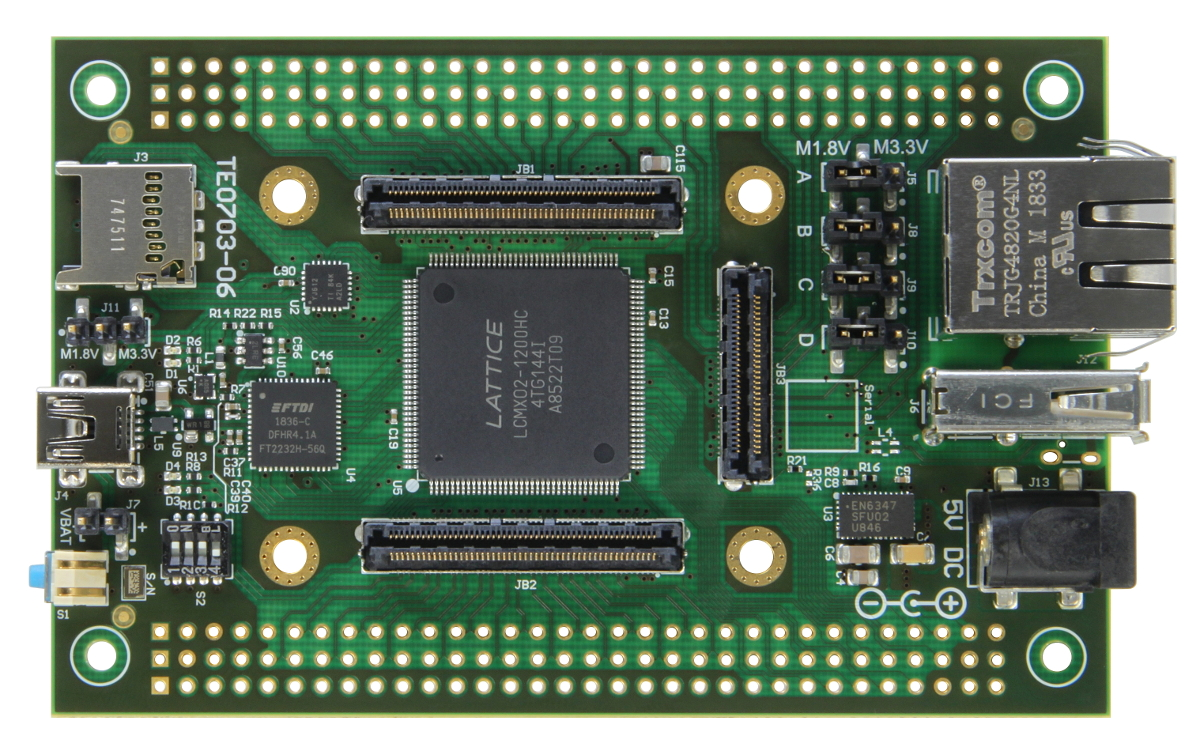
\includegraphics[scale=0.23]{imagenes/TE0703-06_1.jpg}
    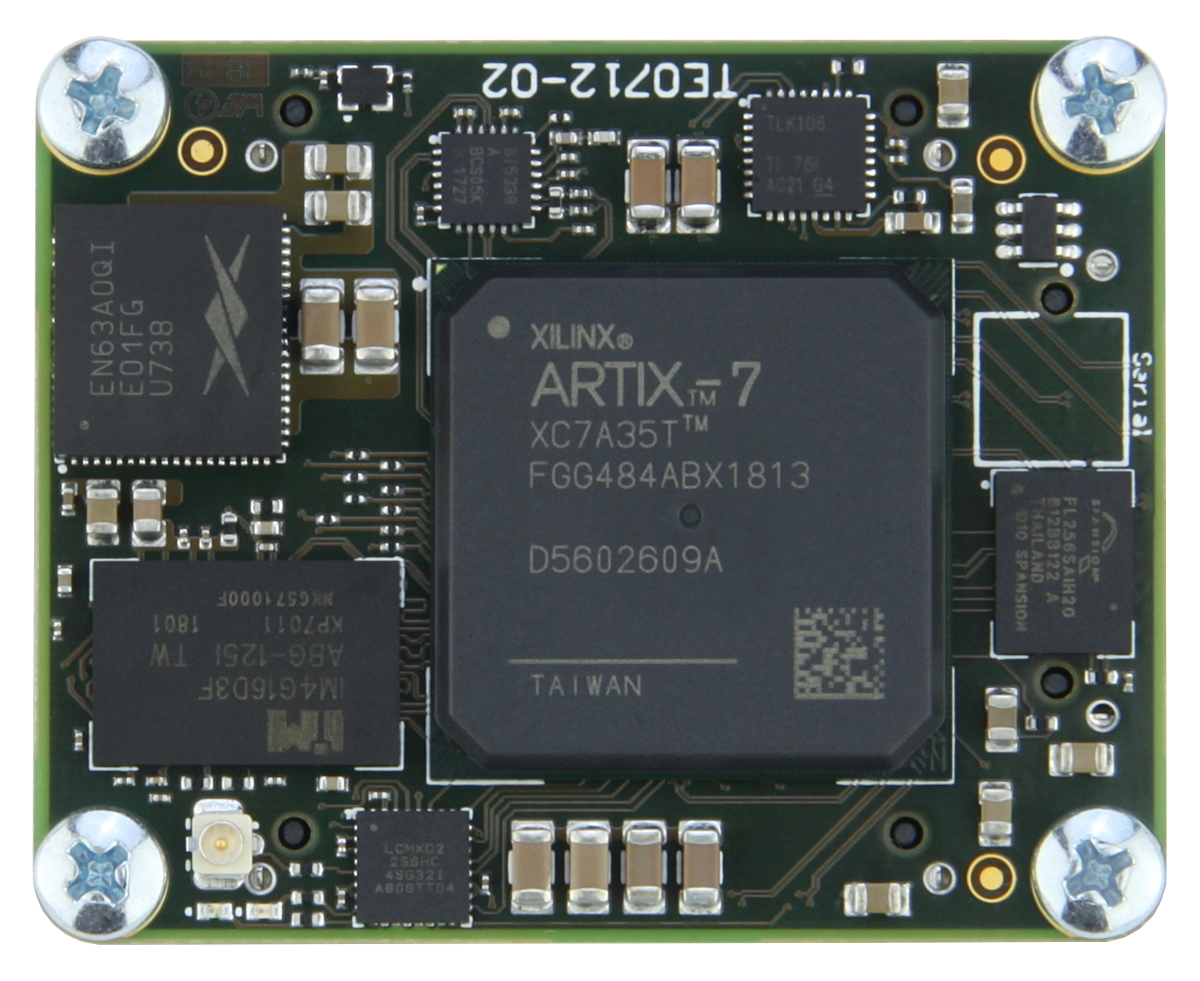
\includegraphics[scale=0.13]{imagenes/TE0712-02-35-2I_1.jpg}
    \caption{Placa de desarrollo y módulo FPGA a utilizar. A la izquierda se ilustra la placa de desarrollo Trenz TR0703\cite{TrenzElectronic2019TR0703Wiki} y a su derecha se ilustra el módulo que va montado en ella: Trenz TR0712\cite{TrenzElectronic2019TR07012Wiki} que contiene una FPGA Artix 7\cite{Xilinx20107DS180}.}
    \label{fig:trenz}
\end{figure}


\par Para esta alternativa de solución se consideran 32 canales de entrada LVDS ya que en el futuro será necesario conectar al menos 2 detectores de 16 canales en una misma FPGA. Para este proyecto en particular se probará el sistema con un solo detector de muones, por lo que la prueba e integración de un segundo detector queda pendiente y no se implementará en esta etapa. La figura \ref{fig:ministgc} ilustra los canales que posee un solo detector de muones de $15cm^2$.

\begin{figure}[H]
    \centering
    \includegraphics[scale=0.5]{imagenes/ministgc.pdf}
    \caption{Esquema de los canales provenientes de un detector Mini sTGC. Posee 8 tiras adyacentes de 15cm de largo por 1cm de ancho para cada eje coordenado. Cada tira emitirá un pulso analógico si una partícula cargada pasa través de ella. Se emitirán también pulsos de menor amplitud para el caso en que la partícula pase por una tira adyacente del mismo eje coordenado dentro de un radio específico. Este detector se posiciona perpendicularmente respecto a la fuente de radiación y en paralelo a (por debajo o por sobre) el sistema de disparo que indicará si la partícula captada corresponde o no a un muón. }
    \label{fig:ministgc}
\end{figure}

\par Las señales generadas por un detector son adaptadas por una tarjeta de interfaz ASD\cite{1999ATLASICs}, ilustrada en la figura \ref{fig:asd}. Esta tarjeta es capaz de capturar 16 señales simultaneas, por lo que es hardware suficiente para captar las señales de ambos ejes de un solo detector de muones.

\begin{figure}[H]
    \centering
    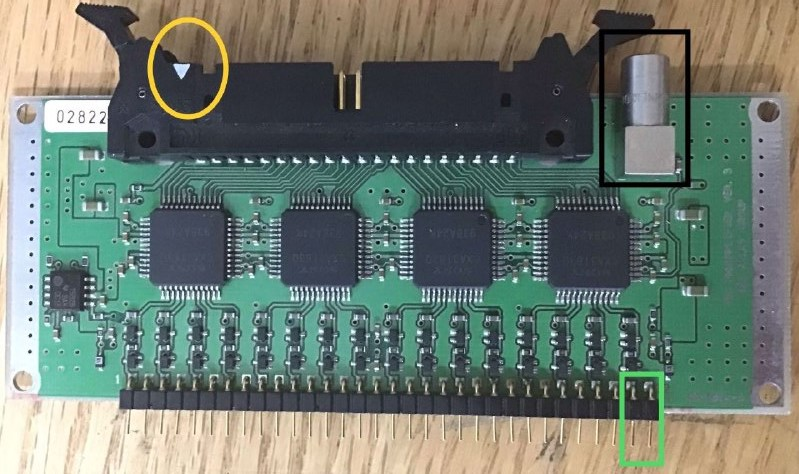
\includegraphics[scale=0.4]{imagenes/asd.jpg}
    \caption{Placa ASD\cite{1999ATLASICs} (Amplificator Shaper Discriminator), encargada de captar los 16 pulsos provenientes de un detector y entregar pulsos digitales asociados a ellos en su salida. El detector se conecta en sus entradas DIP ubicadas en su extremo inferior, mientras que las señales LVDS de salida se ubican en el conector de 40 puertos para cable plano en su extremo superior.}
    \label{fig:asd}
\end{figure}

\begin{figure}[H]
    \centering
    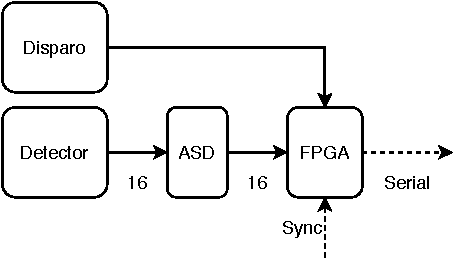
\includegraphics[scale=0.75]{imagenes/fpga1.pdf}
    \caption{Diagrama de bloques utilizando una FPGA como alternativa de solución. Se indica una salida serial para transmitir los resultados del análisis básico a algún procesador o memoria de alguna etapa posterior. La señal de sincronización ``Sync'' tiene como objetivo sincronizar la recolección y procesamiento de eventos, para que estos sean consistentes entre detectores.}
    \label{fig:fpga1}
\end{figure}


\par La idea en esta alternativa de solución es guardar los pulsos provenientes de la placa ASD en memoria temporal hasta la llegada de una señal de disparo. Un módulo que maneja la memoria será el encargado de tomar los pulsos correspondientes al disparo recibido y liberar la memoria de aquellos datos ya leídos u obsoletos, entregando la información útil a una siguiente etapa. Los pulsos aceptados serán entonces relacionados como parte de un mismo eventos y se estimará la duración de estos, generando y guardando así un arreglo de datos con identificador de pulso y duración. La última etapa se encargará de efectuar una operación capaz de determinar la posición del evento a partir de las duraciones medidas y los pulsos detectados, comunicando así un arreglo básico y preprocesado que incluya posición espacial y magnitud aproximada.


\begin{figure}[H]
    \centering
    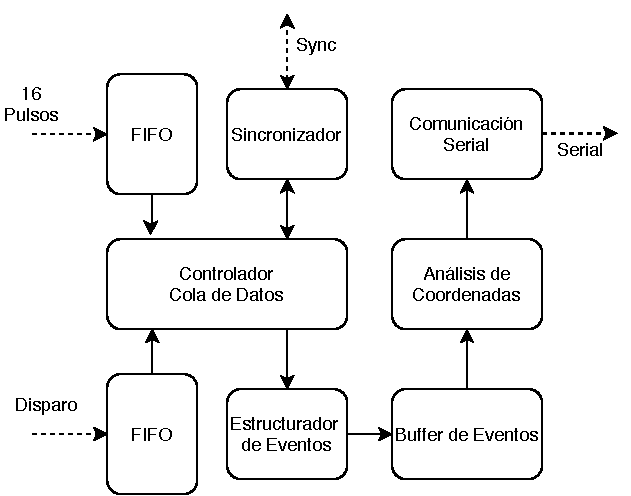
\includegraphics[scale=0.75]{imagenes/fpga2.pdf}
    \caption{Representación de la lógica interna de la FPGA. Se incluye una cola de datos para las señales de disparo, para los pulsos digitales provenientes de la ASD y una memoria de almacenamiento temporal para los eventos ya estructurados. Los bloques controlador, estructurador y análisis cumplen las funciones de aceptar o descartar pulsos, cuantificar anchos de pulso a  los canales asociados y determinar coordenada del cruce de un muón respectivamente.}
    \label{fig:fpga2}
\end{figure}

\par Se espera que para lograr el escalamiento se incluya una señal para mantener la lectura de eventos sincronizada entre distintas FPGA. Además, se deberá incluir un modulo de comunicación para entregar la información captada a una etapa posterior con un análisis más detallado, encargado de reunir todos los eventos de diferentes FPGAs.


\newpage
\section{Conclusión}
\par Luego de presentar y evaluar diferentes alternativas de solución, el análisis indica que la mejor solución corresponde a implementar el sistema en una FPGA, obteniendo un resultado de 8.4 puntos según los criterios de selección. Esta alternativa fue precisamente la que se ha considerado desde un principio y coincide con ser la tecnología más utilizada dentro del desarrollo de sistemas de adquisición para física de partículas\cite{Basiladze2017Methods1}\cite{Basiladze2017Methods2}.
\par Esta alternativa fue seleccionada por sobre las demás debido a su destacado desempeño, ya que cuenta con mayor frecuencia de reloj disponible, gran cantidad de recursos y suficientes puertos LVDS. Este último requerimiento es necesario para recibir los pulsos digitales capturados por la interfaz ASD provenientes del detector, los cuales se emiten bajo el estándar LVDS para transmisión de señales diferenciales.
\par Destaca también esta alternativa al ser una plataforma flexible, en sentido de brindar las posibilidades de adaptar el diseño propuesto sin tener que adquirir nuevo equipamiento. Esta versatilidad es intrínseca de las FPGAs, las cuales se caracterizan por permitir un gran control en el diseño del hardware a bajo nivel.
\par Luego de este trabajo de selección y detalle de la solución, ya se encuentran definidos los objetivos principales del proyecto y los esquemas generales del diseño a implementar para cumplir con ellos. Con la información presentada en la sección \ref{alternativa} es posible comenzar las etapas de planificación y posterior ejecución del proyecto, para desarrollar así un sistema de adquisición de datos para detectores de muones escalable basado en FPGA.
